%%%%%%%%%%%%%%%%%%%%%%%%%% lecture-7
%\begin{frame}[shrink]
%  \frametitle{lecture-7 主要内容}
%  \framesubtitle{循环结构程序设计举例}
%  \tableofcontents[hideallsubsections]
%\end{frame}

\section{循环结构程序设计举例}

\begin{frame}[shrink,fragile]
$[$例5.7$]$用公式$\frac{\pi}{4}\approx 1-\frac{1}{3}+\frac{1}{5}-\frac{1}{7}+\cdots$求$\pi$的近似值, 直到发现某一项的绝对值小于$10^{-6}$为止(该项不累加)。\\
~\\
\begin{columns}
\column{0.7\textwidth}
解题思路:  找规律
\begin{enumerate}
	\item 每项的分子都是1。
	\item 后一项的分母是前一项的分母加2。
	\item 第1项的符号为正,从第2项起,每一项的符号与前一项的符号相反。
	在每求出一项后,检查它的绝对值是否大于或等于$10^{-6}$。
\end{enumerate}
\column{0.3\textwidth}
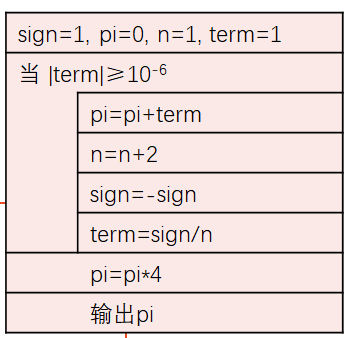
\includegraphics[scale=0.3]{pi}
\end{columns}
\end{frame}

\begin{frame}[shrink,fragile]
\begin{lstlisting}
#include <stdio.h>
#include <math.h> //程序中用到数学函数fabs,应包含头文件math.h
int main()
{
  int sign=1; //sign用来表示数值的符号
  double pi=0.0,n=1.0,term=1.0; //pi开始代表多项式的值,最后代表$\pi$的值, n代表分母,term代表当前项的值
  while(fabs(term)>=1e-6) //检查当前项term的绝对值是否大于或等于$10^{-6}$
  {
    pi=pi+term; //把当前项term累加到pi中
    n=n+2;      //n+2是下一项的分母 
    sign=-sign; //sign代表符号,下一项的符号与上一项符号相反
    term=sign/n; //求出下一项的值term
  }
  pi=pi*4; //多项式的和pi乘以4,才是$\pi$的近似值
  printf("pi=%10.8f\n",pi);  //输出$\pi$的近似值  
  return 0;
}
\end{lstlisting}
\end{frame}

\begin{frame}[shrink,fragile]
\small
$[$例5.8$]$求Fibonacci(斐波那契)数列的前40个数。这个数列有如下特点: 第1, 2两个数为1, 1。从第3个数开始,该数是其前面两个数之和。即该数列为1,1,2,3,5,8,13,\dots,用数学方式表示为:
\[
\begin{cases}
F_1=1 & (n=1)\\
F_2=1 & (n=2)\\
F_n=F_{n-1}+F_{n-2} & (n\ge 3)\\
\end{cases}
\]
\begin{columns}
	\column{0.4\textwidth}
	这是一个有趣的古典数学问题: 有一对兔子,从出生后第3个月起每个月都生一对兔子。小兔子长到第3个月后每个月又生一对兔子。假设所有兔子都不死,问每个月的兔子总数为多少?
	\column{0.6\textwidth}
	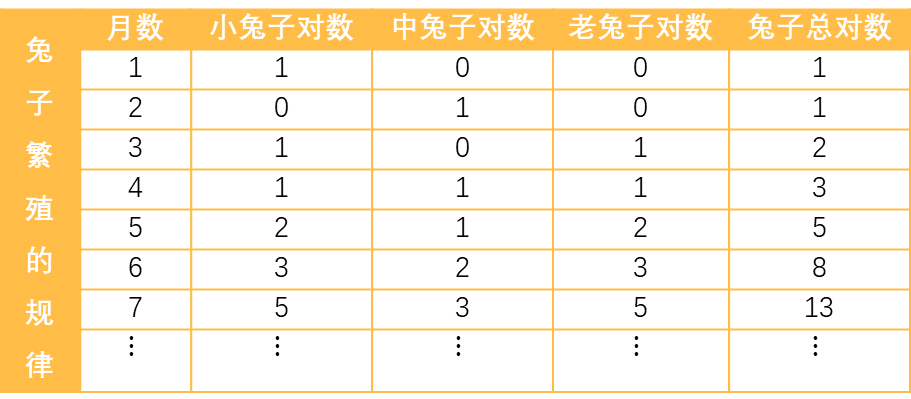
\includegraphics[scale=0.45]{Fn}
	\scriptsize
	不满1个月的为小兔子,满1个月不满2个月的为中兔子,满2个月以上的为老兔子。
\end{columns}
\end{frame}

\begin{frame}[shrink,fragile]
解法一: 利用递推(迭代)公式: $F_1=F_2=1; F_3=F_1+F_2; F_1=F_2; F_2=F_3; $
\begin{columns}
	\column{0.6\textwidth}
	\begin{lstlisting}
    #include <stdio.h>
    int main()
    {
        int f1=1,f2=1,f3;
        int i;
        printf("%12d\n%12d\n",f1,f2);
        for(i=1; i<=38; i++)
        {
            f3=f1+f2;
            printf("%12d\n",f3);
            f1=f2;
            f2=f3;
        }
        return 0;
    }
    \end{lstlisting}
	\column{0.3\textwidth}
	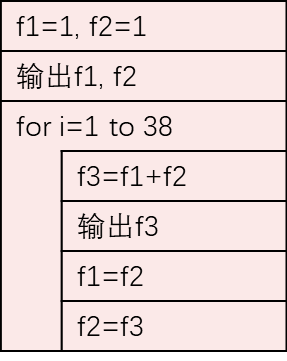
\includegraphics[scale=0.6]{Fn1}\\
	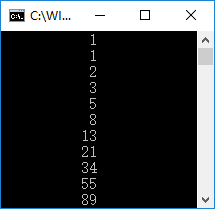
\includegraphics[scale=0.6]{Fno1}
\end{columns}
\end{frame}

\begin{frame}[shrink,fragile]
解法二: 利用递推(迭代)公式: $F_1=F_2=1; F_1=F_1+F_2; F_2=F_1+F_2; $
\begin{columns}
	\column{0.5\textwidth}
\begin{lstlisting}
#include <stdio.h>
int main()
{
  int f1=1,f2=1;
  int i;
  for(i=1; i<=20; i++)
  {
    printf("%12d%12d",f1,f2);
    if(i%2==0) // 等效 if(!(i%2)) 
       printf("\n");
    f1=f1+f2;
    f2=f2+f1;
  }
  return 0;
}
\end{lstlisting}
	\column{0.4\textwidth}
	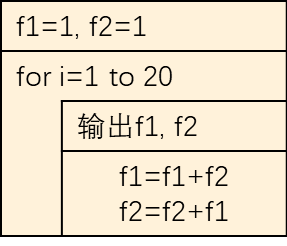
\includegraphics[scale=0.6]{Fn2}\\
	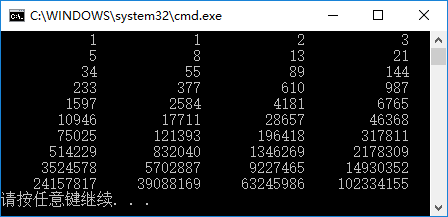
\includegraphics[scale=0.6]{Fno2}
\end{columns}
\end{frame}

\begin{frame}[shrink,fragile]
\small
$[$例5.9$]$输入一个大于3的整数n,判定它是否为素数(prime,又称质数)。
\centering
\begin{columns}
	\column{0.65\textwidth}
\begin{lstlisting}
#include <stdio.h>
int main()
{
  int n,i;
  printf("please enter a integer number,n=?");
  scanf("%d",&n);
  for (i=2;i<n;i++)
    if(n%i==0) break;
  if(i<n) // for提前结束
    printf("%d is not a prime number.\n",n);
  else // for正常结束
    printf("%d is a prime number.\n",n);
  return 0;
}
\end{lstlisting}
	\column{0.3\textwidth}
	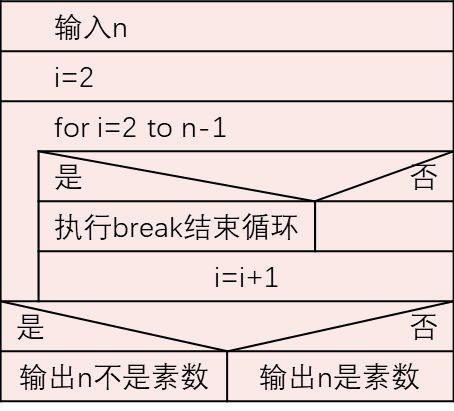
\includegraphics[scale=0.5]{prime}
\end{columns}
\textcolor{blue}{只要在循环结束后检查循环变量i的值,就能判定循环是提前结束还是正常结束的。从而判定n是否为素数。这种判断循环结束的方法以后会常用到。}
\end{frame}

\begin{frame}[shrink,fragile]
\small
\textbf{\textcolor{blue}{优化: }} $n$不必被$2\sim (n-1)$内的各整数去除,只须将$n$被$2\sim\sqrt{n}$之间的整数除即可。因为n的每一对因子, 必然有一个小于n, 另一个大于n。
%\centering
\begin{lstlisting}
#include <stdio.h>
#include <math.h>
int main()
{
   int n,i,k;
   printf("please enter a integer number,n=?");
   scanf("%d",&n);
   k=sqrt(n); // 自动转换为整数(不会四舍五入), 相当于k=(int)sqrt(n);
   for (i=2;i<=k;i++)
     if(n%i==0) break;
   if(i<=k) 
      printf("%d is not a prime number.\n",n);
   else 
      printf("%d is a prime number.\n",n);
   return 0;
}
\end{lstlisting}
\end{frame}

\begin{frame}[shrink,fragile]
\small
\textbf{\textcolor{blue}{使用标志变量, 判断循环结束条件。}}
%\centering
\begin{lstlisting}
int n,i,k,flag=1; // flag: 标志变量
k=sqrt(n); // 自动转换为整数(不会四舍五入), 相当于k=(int)sqrt(n);
for (i=2;i<=k;i++)
   if(n%i==0) { flag=0; break; }
if(!flag) // for提前结束
   printf("%d is not a prime number.\n",n);
else // for正常结束
   printf("%d is a prime number.\n",n);
\end{lstlisting}
\pause
\rule{\textwidth}{1pt} %水平线
\begin{lstlisting}
int n,i,k,flag=1; // flag: 标志变量
k=sqrt(n); // 自动转换为整数(不会四舍五入), 相当于k=(int)sqrt(n);
for (i=2;i<=k && flag;i++) // 比较与上面for的不同
   if(n%i==0) { flag=0; }
if(!flag) 
   printf("%d is not a prime number.\n",n);
else 
   printf("%d is a prime number.\n",n);
\end{lstlisting}
\end{frame}

\begin{frame}[shrink,fragile]
\small
$[$例5.10$]$求$100\sim 200$间的全部素数。
\pause
\begin{lstlisting}
#include <stdio.h>
#include <math.h>
int main()
{
  int n,i,k;
  for (n=101;n<=200;n+=2) //n从101变化到200, 对每个奇数n进行判定
  {
     k=sqrt(n); // 自动转换为整数(不会四舍五入), 相当于k=(int)sqrt(n);
     for(i=2;i<=k;i++)
        if(n%i==0) break;
     if(i>k) 
        printf("%d ",n);
  }
  printf("\n");
  return 0;
}
\end{lstlisting}
\end{frame}

\begin{frame}[shrink,fragile]
$[$例5.11$]$译密码。为使电文保密,往往按一定规律将其转换成密码,收报人再按约定的规律将其译回原文。例如,可以按以下规律将电文变成密码:将字母A变成字母E,a变成e,即变成其后的第4个字母,W变成A,X变成B,Y变成C,Z变成D。
\begin{center}
\begin{tikzpicture}[>=latex, shorten >=1pt,node distance=1cm, on grid, auto,semithick,initial text=, every state/.style={draw=none,minimum size=0.5cm,outer sep=0pt,inner sep=1pt},every label/.style={outer sep=0pt,inner sep=3pt,},every fit/.style={rectangle,rounded corners=3mm,inner xsep=5mm,inner ysep=3mm,outer sep=2pt},font=\small]
\node[state,label={below:0}] (a) {A};
\node[state,label={below:1}] (b) [right= of a] {B};
\node[state,label={below:2}] (c) [right= of b] {C};
\node[state,label={below:3}] (d) [right= of c] {D};
\node[state,label={below:4}] (e) [right= of d] {E};
\node[state,label={below:$\cdots$}] (dot) [right=2cm of e] {$\cdots$};
\node[state,label={below:22}] (w) [right= of dot] {W};
\node[state,label={below:23}] (x) [right= of w] {X};
\node[state,label={below:24}] (y) [right= of x] {Y};
\node[state,label={below:25}] (z) [right= of y] {Z};
\node[] at($(a)+(-0.7,-0.4)$) {Index};
\path[->]
(a) edge[bend right=45] (e)
(w) edge[bend right,dashed,blue] (a)
(x) edge[bend left=45,dashed,red] (b)
;
\end{tikzpicture}
\end{center}
\end{frame}

\begin{frame}[shrink,fragile,plain]
\begin{tikzpicture}[>=latex, shorten >=1pt,node distance=0.7cm, on grid, auto,semithick,initial text=, every state/.style={draw=none,minimum size=0.5cm,outer sep=0pt,inner sep=1pt},every label/.style={outer sep=0pt,inner sep=3pt,},every fit/.style={rectangle,rounded corners=3mm,inner xsep=5mm,inner ysep=3mm,outer sep=2pt},font=\small]
\node[state,label={below:0}] (a) {A};
\node[state,label={below:1}] (b) [right= of a] {B};
\node[state,label={below:2}] (c) [right= of b] {C};
\node[state,label={below:3}] (d) [right= of c] {D};
\node[state,label={below:4}] (e) [right= of d] {E};
\node[state,label={below:$\cdots$}] (dot) [right=2cm of e] {$\cdots$};
\node[state,label={below:22}] (w) [right= of dot] {W};
\node[state,label={below:23}] (x) [right= of w] {X};
\node[state,label={below:24}] (y) [right= of x] {Y};
\node[state,label={below:25}] (z) [right= of y] {Z};
\node[] at($(a)+(-0.7,-0.4)$) {Index};
%\node[blue] at($(z)+(2,-0.4)$) {\lstinline|index=c-'A'|};
\path[->]
(a) edge[bend right=45] (e)
(w) edge[bend right,dashed,blue] (a)
(x) edge[bend left=45,dashed,red] (b)
;
\node[anchor=north west,text width=0.9\textwidth,rounded corners,draw] at($(a)+(-0.5,-1.4)$) {
	\vspace{-0.4cm}
	\begin{lstlisting}
	char c;
	c=getchar(); //输入一个字符给字符变量c
	while(c!='\n') //检查c的值是否为换行符'\n'  
	{
		if((c>='a' && c<='z') || (c>='A' && c<='Z')) //c如果是字母
		{
			if((c>='W' && c<='Z') || (c>='w' && c<='z')) c = c-22; //如果是26个字母中最后4个字母之一就使c-22
			else  c =c + 4;   //如果是前面22个字母之一,就使c + 4
		}
		printf("%c",c); //输出已改变的字符
		c=getchar();    //再输入下一个字符给字符变量c
	}
	printf("\n");
	\end{lstlisting}
};
\end{tikzpicture}
\end{frame}

\note{a,b,c,d,e,$\dots$,v(第22个字符),w(c-22),x(c-22),y(c-22),z(c-22)}

\begin{frame}[shrink,fragile,plain]
\begin{tikzpicture}[>=latex, shorten >=1pt,node distance=0.7cm, on grid, auto,semithick,initial text=, every state/.style={draw=none,minimum size=0.5cm,outer sep=0pt,inner sep=1pt},every label/.style={outer sep=0pt,inner sep=3pt,},every fit/.style={rectangle,rounded corners=3mm,inner xsep=5mm,inner ysep=3mm,outer sep=2pt},font=\small]
\node[state,label={below:0}] (a) {A};
\node[state,label={below:1}] (b) [right= of a] {B};
\node[state,label={below:2}] (c) [right= of b] {C};
\node[state,label={below:3}] (d) [right= of c] {D};
\node[state,label={below:4}] (e) [right= of d] {E};
\node[state,label={below:$\cdots$}] (dot) [right=2cm of e] {$\cdots$};
\node[state,label={below:22}] (w) [right= of dot] {W};
\node[state,label={below:23}] (x) [right= of w] {X};
\node[state,label={below:24}] (y) [right= of x] {Y};
\node[state,label={below:25}] (z) [right= of y] {Z};
\node[] at($(a)+(-0.7,-0.4)$) {Index};
\node[blue] at($(z)+(1.6,-0.4)$) {另解:\lstinline|index=c-'A'|};
\path[->]
(a) edge[bend right=45] (e)
(w) edge[bend right,dashed,blue] (a)
(x) edge[bend left=45,dashed,red] (b)
;
\node[anchor=north west,text width=0.9\textwidth,rounded corners,draw] at($(a)+(-0.5,-1.4)$) {
	\vspace{-0.4cm}
	\begin{lstlisting}
	char c;
	c=getchar(); //输入一个字符给字符变量c
	while(c!='\n') //检查c的值是否为换行符'\n'  
	{
		if((c>='A' && c<='Z')) //c如果是大写字母
			c='A'+(c-'A'+4)%26;
		else if((c>='a' && c<='z')) //c如果是小写字母
			c='a'+(c-'a'+4)%26;
		printf("%c",c); //输出已改变的字符
		c=getchar();    //再输入下一个字符给字符变量c
	}
	printf("\n");
	\end{lstlisting}
};
\end{tikzpicture}
\end{frame}

\begin{frame}[shrink,fragile]{在循环条件中接收输入的字符是一种常见技巧}
\begin{tikzpicture}[>=latex, shorten >=1pt,node distance=0.7cm, on grid, auto,semithick,initial text=, every state/.style={draw=none,minimum size=0.5cm,outer sep=0pt,inner sep=1pt},every label/.style={outer sep=0pt,inner sep=3pt,},every fit/.style={rectangle,rounded corners=3mm,inner xsep=5mm,inner ysep=3mm,outer sep=2pt},font=\small]
\node[text width=\textwidth,rounded corners,draw] {
	\vspace{-0.4cm}
	\begin{lstlisting}
	char c;
	while((c=getchar())!='\n') //首先从键盘接收一个字符c, 再检查c的值是否为换行符'\n'  
	{
		if((c>='A' && c<='Z')) //c如果是大写字母
			c='A'+(c-'A'+4)%26;
		else if((c>='a' && c<='z')) //c如果是小写字母
			c='a'+(c-'a'+4)%26;
		printf("%c",c); //输出已改变的字符
	}
	printf("\n");
	\end{lstlisting}
};
\end{tikzpicture}
\end{frame}
